a) Completar la tabla
\begin{center}
	\begin{table}[htbp]
		\begin{center}
			\begin{tabular}{|c|c|c|c|c|c|c|c|}
				\hline
				$I$ & $n_{i}$ & $N_{i}$ & $f_{i}$ & $F_{i}$ & $c_{i}$ & $a{i}$ & $h_{i}$\\\hline
				(8300, 9300] & 2 & 2 & 2/18 & 2/18 & 8800 & 1000 & 0.002/18 \\ \hline
				(9300, 10200] & 3 & 5 & 3/18 & 5/18 & 9750 & 900 & 1/5400 \\ \hline
				(10200, 11300] & 5 & 10 & 5/18 & 10/18 & 10750 & 1100 & 1/3960 \\ \hline
				(11300, 12700] & 2 & 12 & 2/18 & 12/18 & 12000 & 1400 & 1/12600 \\ \hline
				(12700, 13500] & 4 & 16 & 4/18 & 16/18 & 13100 & 800 & 0.005/18 \\ \hline
				(13500, 14500] & 2 & 18 & 2/18 & 1 & 14000 & 1000 & 0.002/18\\ \hline
			\end{tabular}
		\end{center}
	\end{table}
\end{center}

b) Representar la distribución mediante un histograma, poligonal de frecuencias y curva de
distribución.

\begin{center}
    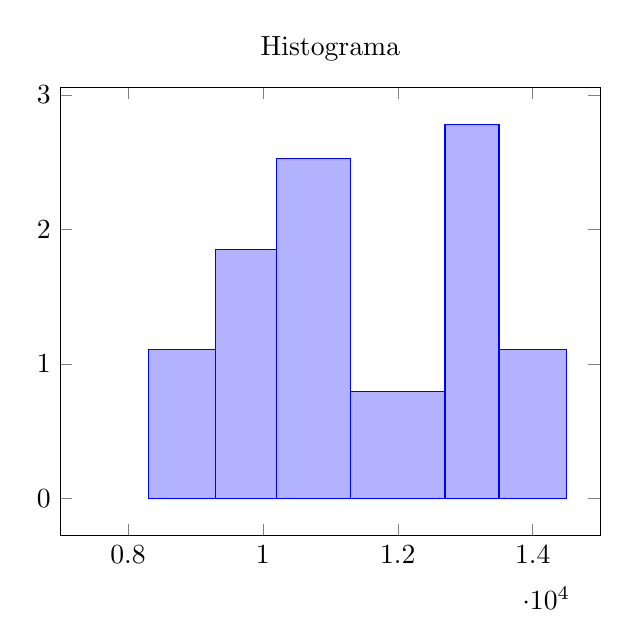
\begin{tikzpicture}
        \begin{axis}[
            title = {Histograma},
            xmin=7000, xmax=15000,
            area style
            ]
        \addplot+[ybar interval,mark=no] plot coordinates {
        (8300, 1.111)
        (9300, 1.852)
        (10200, 2.525)
        (11300, 0.794)
        (12700, 2.777)
        (13500, 1.111)
        (14500, 0)
        };
        \end{axis}
    \end{tikzpicture}
\end{center}

\vspace{5mm}
\begin{center}
    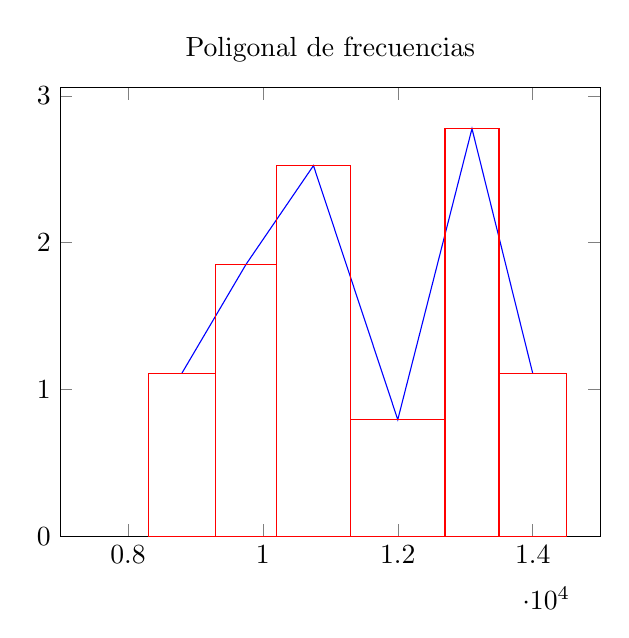
\begin{tikzpicture}
        \begin{axis}[
        title={Poligonal de frecuencias},
        xmin=7000, xmax=15000,
        ymin=0
        ]

        \addplot[
        color=blue,
        ]
        coordinates {
        (8800, 1.111)
        (9750, 1.852)
        (10750, 2.525)
        (12000, 0.794)
        (13100, 2.777)
        (14000, 1.111)
        };
        [
        ymin=0, ymax=11,
        minor y tick num = 4,
        area style,
        ]
        \addplot+[ybar interval,mark=no] plot coordinates {
        (8300, 1.111)
        (9300, 1.852)
        (10200, 2.525)
        (11300, 0.794)
        (12700, 2.777)
        (13500, 1.111)
        (14500, 1.111)
        };
        \end{axis}
    \end{tikzpicture}
\end{center}

\begin{center}
    \begin{tikzpicture}
        \begin{axis}[
        title={Curva de distribución},
        xmin=7000, xmax=15000,
        ymin=-0.1, ymax=1.2,
        xtick={1/18, 5/18, 10/18, 12/18, 16/18, 1},
        ytick={0,0.2,0.4,0.6,0.8,1},
        legend pos=north west,
        ymajorgrids=false,
        grid style=dashed,
        ]

        \addplot[
        color=blue,
        ]
        coordinates {
        (700,0)
        (8300,0)
        (9300, 2/18)
        (10200, 5/18)
        (11300,10/18)
        (12700,12/18)
        (13500,16/18)
        (14500,1)
        (15000,1)
        }; 
        \end{axis}
    \end{tikzpicture}
\end{center} \\

c) ¿Cuántas comunidades presentan una renta menor o igual que 12700 euros? ¿Y cuántas superior a 11300 euros?

Como podemos ver en la tabla, las comunidades que presentan una renta menor o igual a 12700 corresponden con $N_{4}$, es decir, 12 comunidades.
Las comunidades con una renta superior a 11300 corresponderían con la suma de las comunidades de los intervalos superiores, es decir, a la suma de $n_{4}$, $n_{5}$ y $n_{6}$. Finalmente, el resultado a esta última pregunta es 8 comunidades.
